\section{Test Images}

In order to test our implementations, we have choose 4 images (figure \ref{fig:Input-images}), extensive experiments have been performed in each one, but more representative results are shown in this report. Complete results can be found in $output$ directory after running $make$ command. For the blending experiment, extra images are used. 

The execution time of the $make$ script may take a while.

\begin{figure}[h!]
\centering
\begin{subfigure}{0.5\textwidth}
  \centering
  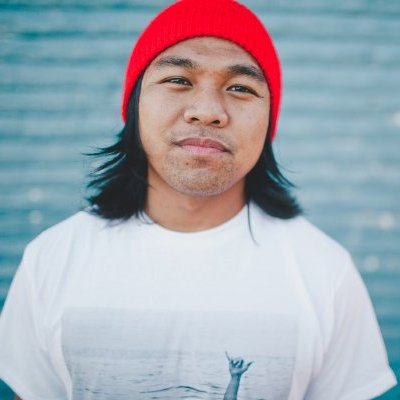
\includegraphics[width=0.5\linewidth]{input/p1-1-0.jpg}
  \caption{Input p1-1-0.jpg, 400x400 pixels}
\end{subfigure}%
\begin{subfigure}{0.5\textwidth}
  \centering
  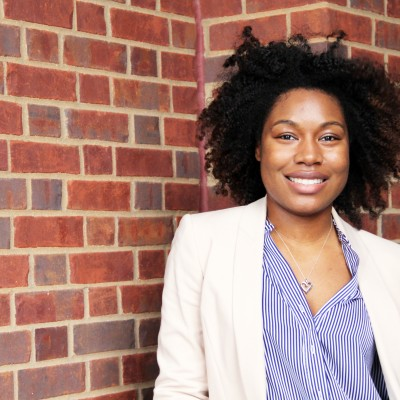
\includegraphics[width=0.5\linewidth]{input/p1-1-1.jpg}
  \caption{Input p1-1-1.jpg, 400x400 pixels}
\end{subfigure}
\begin{subfigure}{0.5\textwidth}
  \centering
  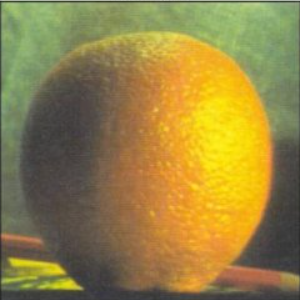
\includegraphics[width=0.5\linewidth]{input/p1-1-2.png}
  \caption{Input p1-1-2.jpg, 300x300 pixels}
\end{subfigure}%
\begin{subfigure}{0.5\textwidth}
  \centering
  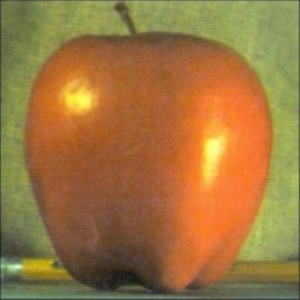
\includegraphics[width=0.5\linewidth]{input/p1-1-3.png}
  \caption{Input p1-1-3.jpg, 300x300 pixels}
\end{subfigure}
 \caption{Images used in experiments}
\label{fig:Input-images}
\end{figure}


